% !TEX root = ../main.tex
\subsection{FMT Alignment}
\label{ssec::fmt_alignment}
% --+ Why is it needed +--------------------------------------------------------
    While in a perfect world the target and each detector would be installed precisely where they are needed, in the real world there is an unavoidable misalignment in their positions.
    This misalignment needs to be addressed and included into reconstruction:
    the software needs to be aware of where a detector is positioned in relation to the target to provide meaningful results.

    In the CLAS collaboration, the Calibration and Commissioning group (CalCom) is in charge of the alignment and calibration of each detector.
    Shifts and rotations that need to be applied for alignment are included in the Calibration and Conditions Database (CCDB), which is then read in reconstruction. % NOTE. A citation would be cool.

    The main goals of alignment work were three:
    First, to provide FMT alignment tables to Run Group F (RG-F) so that they may be used in reconstruction.
    Second, to check if the resolution improvement from FMT is good enough to justify the extra material added to the CLAS12 detector.
    Finally, to provide detailed information about these improvements so that Run Group E (RG-E) and other run groups can choose if they will include the detector to their runs.

% --+ Definitions +-------------------------------------------------------------
    Alignment shifts can be made in any of the three global axes:
    $z$, which is concentric to the beamline, $x$, which is parallel to the ground, and $y$, which points up from the ground.
    Then, alignment rotations can be done in any of these axes, and for the purposes of this work will be referred to as $\phi$ rotation (roll), when they're done around the $z$ axis, and pitch and yaw when they're done around the $x$ and $y$ axes respectively.

    To measure misalignment, we define a the Distance Of Closest Approach (DOCA) between a reconstructed DC track and an FMT cluster as a \textbf{Residual}.
    Due to each layer's geometry (refer to figure \ref{fig::fmt_geometry}), only the residuals in a layer's local $y$ axis (perpendicular to the strips) can be measured.
    This means that global $z$ and $\phi$ alignment can be done for each layer independently, but global $x$, global $y$, pitch, and yaw alignment has to be done for the entire detector at once.

% --+ How was it done +---------------------------------------------------------
    \begin{figure}[b!]
        \centering\frame{
        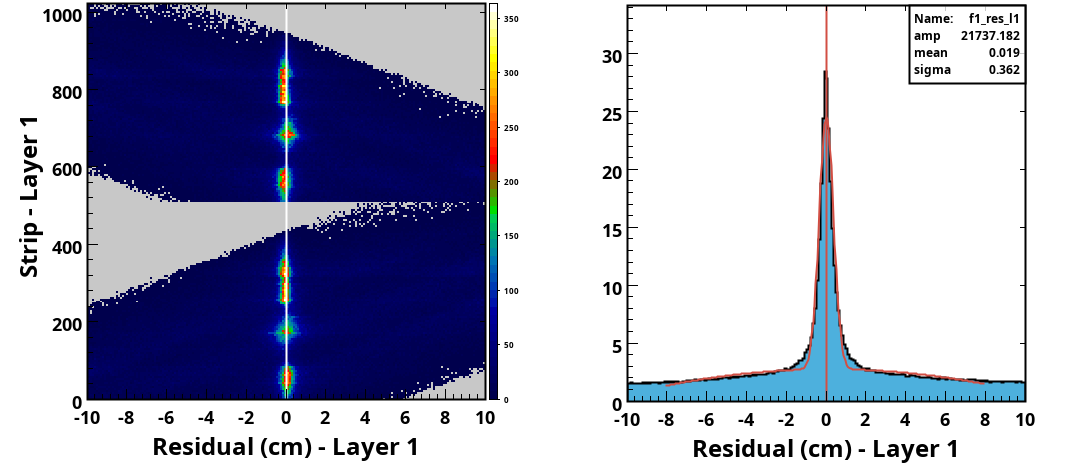
\includegraphics[width=\textwidth]{20res_example.png}}
        \caption[Example FMT residuals plot]{Example FMT residuals plot.
        Source: \hyperlink{github.com/JeffersonLab/clas12alignment}{CLAS12 alignment software}.}
        \label{fig::res_example}
    \end{figure}

    To minimise residuals, they are plotted for a particular shift or rotation in any of the relevant axes.
    An example of such a plot is shown in figure \ref{fig::res_example}.
    Since a Gaussian distribution is to be expected for the residuals, a Gaussian fit is applied to them.
    For $z$ and $\phi$ alignment, the goodness of a fit is evaluated heuristically by comparing their $\sigma$ and choosing the shift with the minimum $\sigma$.
    Then, for $x$, $y$, pitch, and yaw alignment, the goodness of a fit is evaluated heuristically by choosing the fit with the mean closest to $0$.
    The minimums are of course chosen within a healthy error margin.
    Examples of $z$ and $xy$ goodness of fit distributions can be seen in figure \ref{fig::resfit_example}.

    \begin{figure}[t!]
        \centering\frame{
        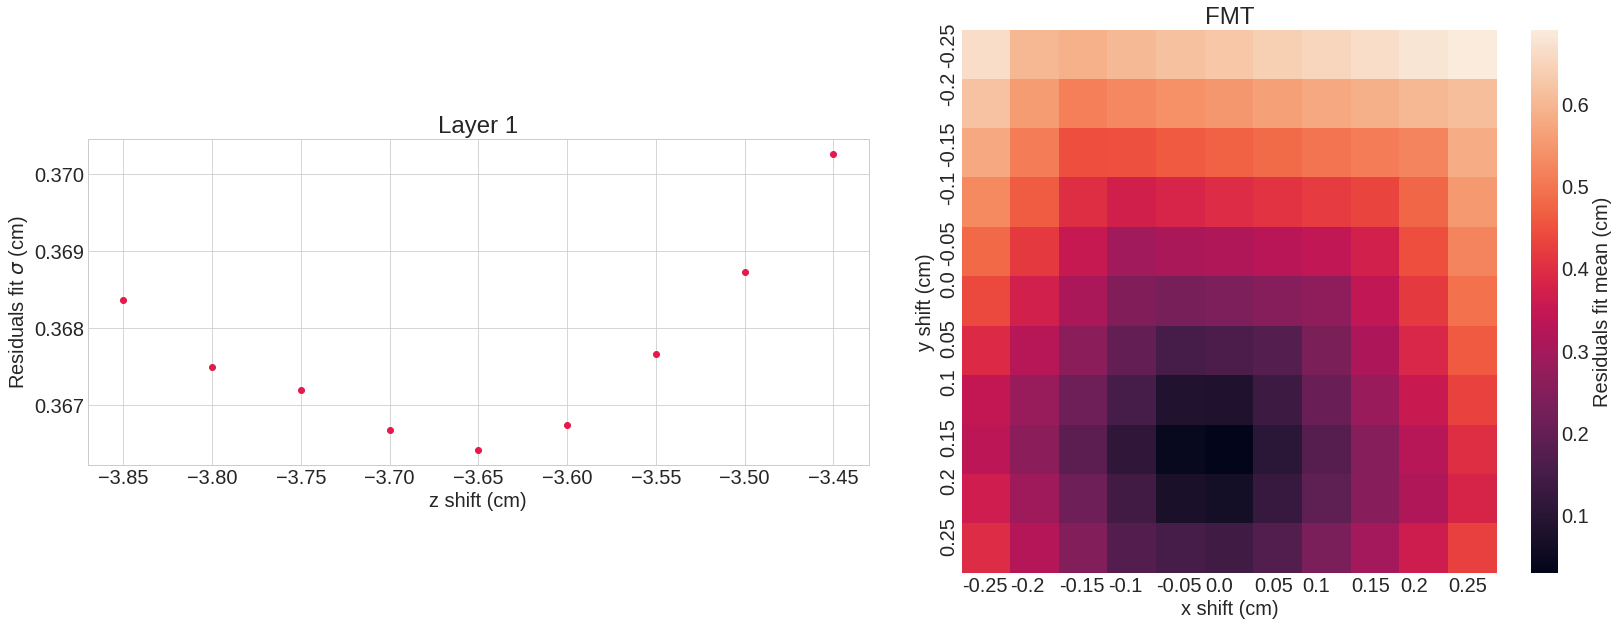
\includegraphics[width=\textwidth]{20resfit_example.png}}
        \caption[Examples of residuals goodness of fit plots]{Examples of residuals goodness of fit plots.
        Source: \hyperlink{github.com/JeffersonLab/clas12alignment}{CLAS12 alignment software}.}
        \label{fig::resfit_example}
    \end{figure}

    % !TEX root = ../main.tex
\subsubsection{Fiducial Cuts}
\label{12.21::fiducial_cuts}
    To mitigate background noise, fiducial cuts are applied to the DC tracks and FMT clusters.
    This process enhances data quality, ensuring more meaningful alignment results.

    For DC tracks, the following cuts are implemented:
    \begin{itemize}
        \item
            $\text{track}.z < \text{layer}.z$:
            This cut removes tracks with a vertex $z$ position further downstream than the FMT layer prior to swimming.
            Such occurrences result from reconstruction errors where the particle origin is outside the target.
        \item
            $\mid\text{track}.z - \text{layer}.z\mid < 0.05 \text{cm}$:
            This eliminates tracks that are too far from the FMT layer after swimming, caused by bugs in the swimmer process that will be discussed in the subsequent section.
        \item
            $5 \text{cm} < \sqrt{x^2 + y^2} < 25 \text{cm}$:
            This removes tracks outside the active region of the layer.
        \item
            $\theta < ~66.42\degree$:
            This excludes tracks with excessively high $\theta$ angles.
            When this occurs, a single particle affects multiple strips, rendering the detector's data less reliable for alignment purposes.
    \end{itemize}

    The implemented fiducial cuts applied to the FMT clusters are:
    \begin{itemize}
        \item
            $50 \text{ns} < \text{T}{\text{min}} < 500 \text{ns}$:
            This cut removes clusters with illogical values for $\text{T}{\text{min}}$, which represents the time of the first hit in the cluster.
        \item
            $\text{size} > 1$ $\&$ $\text{E} > 100$:
            This eliminates small clusters with high energy, as they are generally considered to be of poor quality.
        \item
            $\text{size} < 5$:
            This discards large clusters, as they are deemed to be less useful for analysis purposes.
    \end{itemize}

    \input{12fmt_alignment/22residuals_improvements}

    The procedure described in this section is documented and shared publicly.
    It can be seen at:

    \href{github.com/JeffersonLab/clas12alignment/tree/master/fmt}{\texttt{github.com/JeffersonLab/clas12alignment/tree/master/fmt}}
